% 陪集和同余
% 子群|陪集|左陪集|右陪集|同余|阶|拉格朗日定理

\pentry{子群\upref{Group1}}

\begin{definition}{左陪集}

给定一个群$G$和它的一个子群$H$.从$G$中任意挑一个元素$x$出来,用它来\textbf{左乘} $H$中的每一个元素,得到一个集合$\{x, xh_1, xh_2, \cdots\}$,这里的$h_n$要取遍每一个在$H$中的元素.这个集合,也可以写为$\{xh|h\in H\}$,被叫做\textbf{子群$H$关于元素$x$的左陪集(left coset)},记作$xH$. 

\end{definition}

类似地还可以定义右陪集,不过二者选其一作为代表来研究就可以了,我们习惯上主要研究左陪集.

注意这个表示方法:$xH=\{xh|h\in H\}$.这是一种非常简洁的表达方法,可以理解成$x$逐个左乘$H$中的元素得到的集合,也可以理解成是$x$和$H$之间的一个运算,结果是另一个集合.类似地,我们也可以用群里任意两个子集(不一定要求是子群)$A$和$B$来生成一个新的子集$AB=\{ab|a\in A, b\in B\}$,就是用$A$中的每一个元素去左乘$B$中的每一个元素,得到的所有结果的集合.当然,这种表示方法也可以推广到一切“元素之间可以进行运算的集合”:集合$A$和$B$之间的运算,就是$A$和$B$所有可能的元素运算的结果构成的集合.比如说,考虑到整数集合上可以进行小学所学的乘法和加法运算,我们也可以把$n\mathbb{Z}$的表示方法理解为用$n$去乘全体整数所得到的集合,这个集合在加法下构成群\footnote{在乘法下一般不构成群,除非$n$是素数,在这种情况下$n\mathbb{Z}$配合乘法和加法就构成了最常见的一种有限域.}.

如果$h\in H$,而$H$是一个\textbf{有限群},那么由于封闭性,$hH=H$.这是因为,用$h$去左乘$H$中的一切元素(包括$h$自己),那么一方面由于封闭性,运算结果还是在$H$内部;另一方面由于群运算的唯一性,每一个左乘运算都不相同.这个论断不能简单地用于无限群.

所以,如果我们用$xH$中任意元素$xh_0$来左乘$H$,得到的$xh_0H$仍然是同一个左陪集:$xH=xh_0H$. 所以我们可以用左陪集中的任何一个元素$x'$来作为代表,把这个左陪集写成$x'H$.

特别地,考察这个形式的集合\footnote{其中省略号表示一直列举下去, 但排除与前面重复的元素. 所以这个集合可能是有限的.}:$\{e, h, hh, hhh, hhhh, \cdots\}$. 那么同样地由于封闭性和运算唯一性可知,这个集合还是群$H$的一个子集.特别地,$H$的群运算限制在这个集合上能构成一个循环群(\autoref{Group_ex2}~\upref{Group}).只要我们把$n$个$h$相乘的结果记为$h^n$,$n$个$h^{-1}$相乘的结果记为$h^{-n}$,那么如此生成的循环群就可以用指数的加法运算来处理了.由单个元素可以生成循环群这一概念,我们引入以下定义:

\begin{definition}{阶}
给定一个群$G$和一个$g\in G$,如果存在一个正整数$n$使得$g^n=e$,那么我们称$g$是一个有限阶的元素.特别地,所有满足条件的$n$中最小的那一个,被称为$g$的\textbf{阶(order)}或者\textbf{指数},记为$\opn{ord}g$.特别地,如果任何整数$n$都不能使$g^n=e$,那么记$\opn{ord}g=\infty$;规定$\opn{ord}e=0$.
\end{definition}

\begin{example}{$n\mathbb{Z}$ 的左陪集}\label{coset_ex2}
整数加群的群运算是通常的加法,所以我们可以把元素$k$所在的左陪集记为$k+n\mathbb{Z}$.比如说,当$n$为$6$,$k$为$1$时,$1+6\mathbb{Z}=\{\cdots, -11, -5, 1, 7, 13, \cdots\}$;当$k$为$8$时,$8+6\mathbb{Z}=\{\cdots, -10, -4, 2, 8, 14, \cdots\}=2+6\mathbb{Z}$.

$6\mathbb{Z}$一共有$6$个不同的左陪集;类似地,$n\mathbb{Z}$一共有$n$个不同的左陪集.
\end{example}
注意左陪集不一定是子群, 例如 $1 + 6\mathbb Z$ 中没有单位元.

\begin{example}{$3\mathbb{Z}$的子群和左陪集}\label{coset_ex3}
$3\mathbb{Z}$虽然是$\mathbb{Z}$的子群,但是它也可以从中再分离出子群来.由于$3\mathbb{Z}$的集合是由全体$3$的倍数构成的,因此全体$6$的倍数构成的集合$6\mathbb{Z}$是$3\mathbb{Z}$的真子集,我们已经知道它构成群了.也就是说,$6\mathbb{Z}$既是$\mathbb{Z}$的子群,又是$3\mathbb{Z}$的子群,甚至还是$2\mathbb{Z}$的子群.

从\autoref{coset_ex2} 中我们知道,$6\mathbb{Z}$作为$\mathbb{Z}$的子群,有$6$个左陪集;但作为$3\mathbb{Z}$的左陪集的时候只有 $6/3=2$ 个左陪集.

下图可以形象地表示$\mathbb{Z}$,$3\mathbb{Z}$以及$6\mathbb{Z}$之间的关系,一般的群和子群的关系也可以类似理解.

\begin{figure}[ht]
\centering
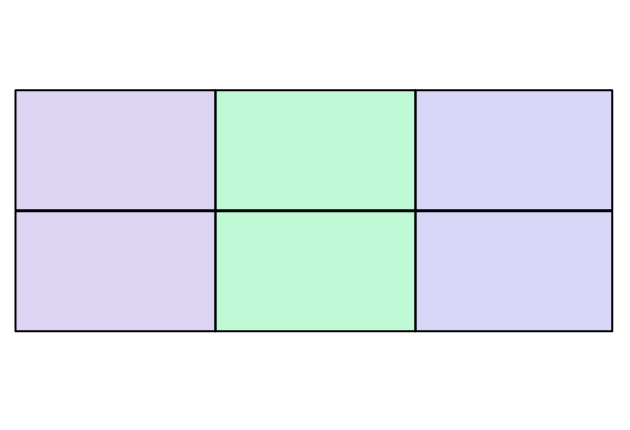
\includegraphics[width=5cm]{./figures/coset_1.png}
\caption{子群和陪集的示意图.整张图表示$\mathbb{Z}$本身;中间的两个绿色区域表示$3\mathbb{Z}$,左边的两个紫色区域表示$1+3\mathbb{Z}$而右边的两个紫色区域表示$2+3\mathbb{Z}$;中间上面的绿色区域表示$6\mathbb{Z}$,而下面的绿色区域表示$3+6\mathbb{Z}$,剩下的四个紫色区域分别表示$6\mathbb{Z}$ 的另外四个左陪集.} \label{coset_fig1}
\end{figure}

在这个图中可以清楚地看到,$3\mathbb{Z}=6\mathbb{Z}\cup(3+6\mathbb{Z})$.这很容易理解,因为$3$的倍数无非两种情况,$6$的倍数或者$6$的倍数再加$3$.

\end{example}

左陪集的意义是将群划分成互不相交的子集,这是一个等价类划分,也就是说,“$x$和$y$属于同一个左陪集”是一个等价关系\upref{Relat}.于是我们有了如下定理: 

\begin{theorem}{}\label{coset_the1}

左陪集划分是一个等价类划分.

\end{theorem}

\textbf{证明}:

给定一个群$G$,两个元素$x, y\in G$,再给定它的一个子集$H$,那么“$y$在左陪集$xH$中”的等价表述,可以是“$y\in xH$”;在这个属于关系两边同时左乘一个$x^{-1}$,还能得到更常用的等价表述:$x^{-1}y\in H$\footnote{如果你不理解为什么可以像解方程一样两边同时乘以一个元素,请再琢磨琢磨上文中$xH$的定义是什么.}.

我们用最后这个等价表述来检查,“在同一个左陪集中”这一关系,是否是等价关系.
\begin{itemize}
\item 自反性:对于任意的$x\in G$,由于$e\in H$,故显然有$x=xe\in xH$.因此$x$和自己在同一个左陪集中.
\item 对称性:如果$x^{-1}y\in H$,由于$H$是个群,故$y^{-1}x=(x^{-1}y)^{-1}\in H$.因此$x$也在左陪集$yH$中.对称性还说明,如果$y$在$xH$中,那么$x$也在$yH$中,因此这两个表述可以合二为一为“$x$,$y$在同一个左陪集中”.
\item 传递性:如果$x^{-1}y\in H$,$y^{-1}z\in H$,那么由于$H$的封闭性,$(x^{-1}y)(y^{-1}x)\in H$,拆开括号后得到$x^{-1}z\in H$. 因此$z$也在$xH$中.
\end{itemize}

到此,我们证明了“在同一个左陪集中”是一个等价关系.由这个等价关系划分的左陪集,是一种等价划分,左陪集彼此互不相交.

\textbf{证毕}

\begin{definition}{同余}
对于群$G$和其子群$H$,如果$x, y\in G$满足$x, y$在同一个左陪集中,那么我们称$x, y$ \textbf{模$H$同余}\footnote{对比整数\upref{intger}中的同余概念.两个“同余”有什么联系吗?}.
\end{definition}

知道了左陪集是等价类,我们很容易发现群的一个优美的结构.在集合论中,子集的基数\upref{Set}可以是任意的,只要它小于等于原集合的基数就可以;但是子群的阶却必须能够整除原群的阶.这就是群论的\textbf{拉格朗日定理(Lagrange's Theorem)}:

\begin{theorem}{拉格朗日定理}\label{coset_the2}

给定群$G$,如果$H$是$G$的子群,那么$|H|$可以整除$|G|$.

\end{theorem}

\textbf{证明}:

假设$x\in G$.根据$xH$的定义,$|xH|\leq|H|$. 又由群运算的唯一性,这个不等式应该取等号:$|xH|=|H|$.所以每个左陪集的基数都一样大.

左陪集彼此不相交,每个元素$x$都属于左陪集$xH$,因此$|G|$等于各个左陪集的基数之和,也就是$|H|$的倍数.

\textbf{证毕}

拉格朗日定理还说明,任何有限群$G$的元素,其指数都是$|G|$的因子.
